
\chapter{ruby\_learnerの概要}

\section{Install/Uninstall}\label{install/uninstall}
InstallとUninstall方法は以下のコマンドを実行することで可能である.
\begin{description}
\def\labelenumi{\arabic{enumi}.}
\tightlist
\item[Install] \$ gem install ruby\_learner
\item[Uninstall] \$ gem uninstall ruby\_learner
\end{description}

\section{ruby\_learnerの全コマンド}\label{commands}
本アプリケーションには多くのコマンドを用意している.その一覧は以下の通りである.
各コマンドの説明は順次行なっていく.
\begin{figure}[H]
\centering
\begin{center}
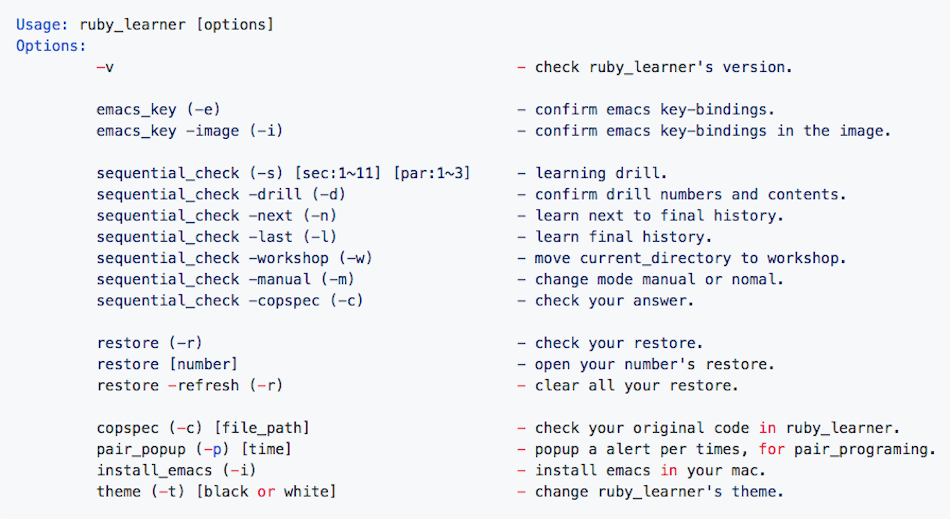
\includegraphics[width=170mm]{../../picture/commands.png}
\end{center}
\caption{ruby\_learnerのコマンド一覧.\label{commands}}
\end{figure}

\section{sequential\_check}\label{sequential_check}
Rubyに関する教材と課題を体系的に学習できるモードである.
教材と課題によって知識のインプットアウトプットを促し,知識の定着を図る.
学習効率を高める為に複数のオプションを用意している.
基本的な学習画面は以下の通り,画面を2分割して上部に回答コード,下部に教材と課題を表示させている.
\begin{figure}[H]
\centering
\begin{center}
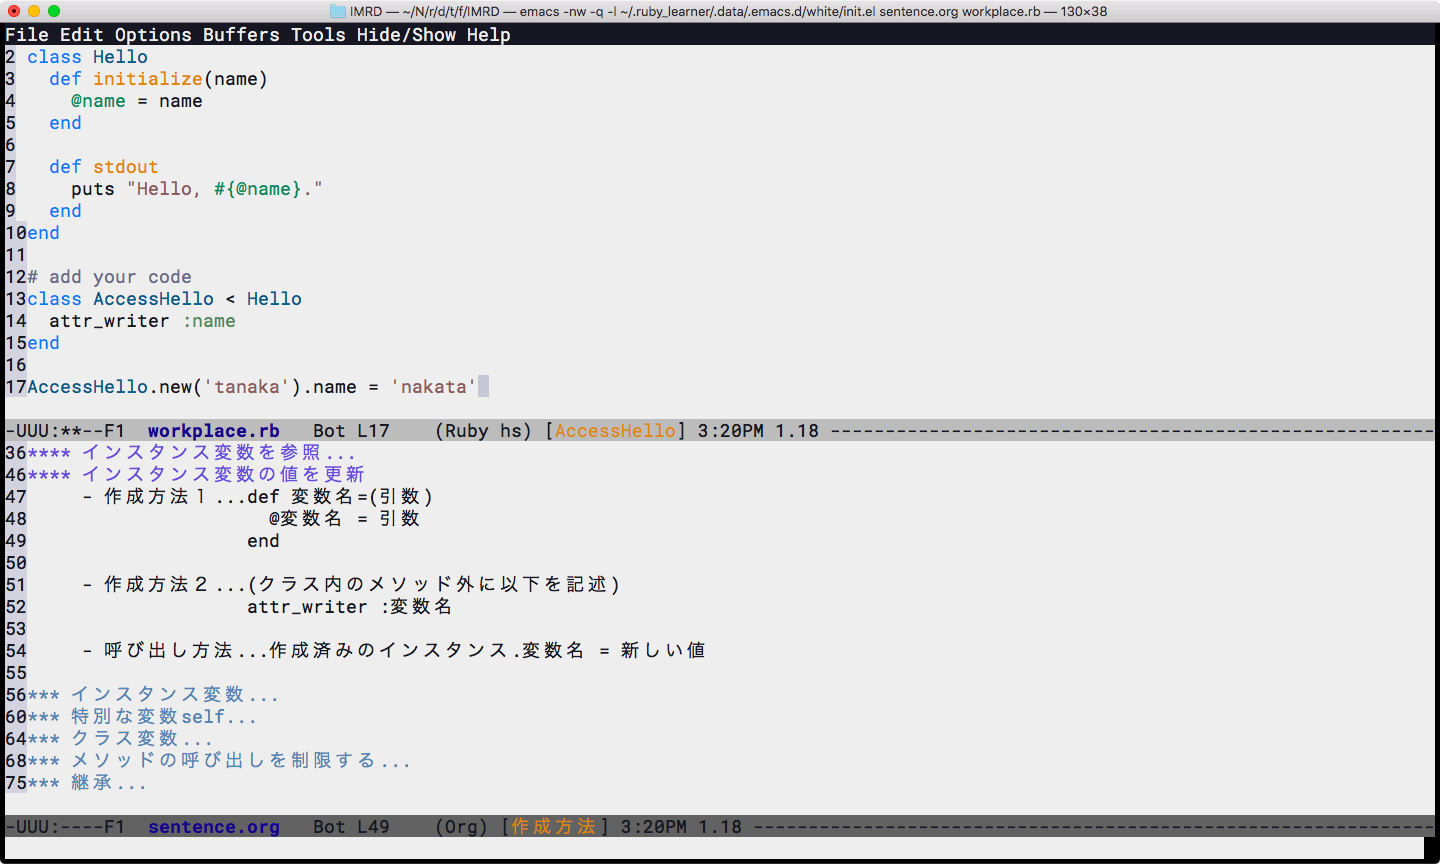
\includegraphics[width=150mm]{../../picture/seq.png}
\end{center}
\caption{sequential\_checkの学習画面.\label{seq}}
\end{figure}
以下はこのモードの詳細である.

\subsection{normal\_mode}\label{nomal_mode}
sequential\_checkが提供する教材と課題の受講方法の1つ.デフォルトではこちらがアクティブになっているが,manual\_modeから切り替える場合は [\$ ruby\_learner -s -m]を実行することで可能である.normal\_modeの状態では,sequential\_checkの学習コマンドの実行時に起こる一連の流れを半自動で実行される.使用者が操作するのは課題回答後のエラー発生時における[回答修正][解答確認][途中終了]の3つのみである.

\subsection{manual\_mode}\label{manual_mode}
sequential\_checkが提供する教材と課題の受講方法の1つ.normal\_modeから切り替える場合には [\$ ruby\_learner -s -m]を実行することで可能である.normal\_modeの状態とは違い,sequential\_checkの学習コマンドの実行後に複数の操作が必要となる.以下にその詳細を記す.
\begin{description}
\def\labelenumi{\arabic{enumi}.}
\tightlist
\item[ディレクトリ構造] 本アプリケーションは初回起動時にホームディレクトリに.ruby\_learnerという隠しディレクトリを作成している.そしてこのディレクトリにはworkshopというディレクトリが存在し,そこで教材と課題の取り組みを行う必要がある.workshop内にはlibとspecという2つのディレクトリがある.libには「教材と課題が一緒になったsentence.org」「使用者が課題の回答を記入するworkplace.rb」「課題の解答が記載されているanswer.rb」の3つのファイルが存在している.specには課題の評価を行うテストファイルが存在している.
  
\item[教材と課題の取り組み] 使用者は手動でemacsを用いてsentence.orgとworkplace.rbを開く必要がある.そのコマンドの一例として[\$ emacs sentence.org workplace.rb]が挙げられる.そしてsentence.orgに記された教材を読み課題を理解した後に,その課題に対する解答をworkplace.rbに記入することで課題に対して回答を行ったと判断される.
\item[評価の実行] 使用者が回答したコードの評価を行うには通常のrspecとrubocopのコマンドを使用する方法以外に,ruby\_learnerがもつコマンドを使用する方法がある.それが[\$ ruby\_learner -s -c]を実行する方法である.このコマンドではnormal\_modeと同様のチェックをworkplace.rbに保存されたコードに行うことができる.このチェックが正常に終了すると,使用者の回答コードが期待される振る舞いとコーディング規約の両面で合格していることとなる.
\end{description}
このモードでは多くの操作を手動で行うことで,開発で用いるディレクトリ構造の把握や実際の開発サイクルの習得が可能である考えられる.

\subsection{last}\label{last}
最新の課題回答を再開することができるオプション..ruby\_learner/workshopのディレクト内に存在するファイル全てに一番最後に回答していた回答コードと教材課題等がコピーされる.一度中断した最新の課題回答を途中から再開できる為,学習効率が向上すると考える.

\subsection{next}\label{next}
最新の課題の次の課題を行うことのできるオプション..ruby\_learner/workshopのディレクト内に存在するファイル全てに次の教材課題等がコピーされる.通常の学習コマンドが[\$ sequential\_check 1 1]の様にセクション番号とパート番号の入力を必要とするのとは違い,[\$ sequential\_check -n]のみで次の課題を行える為,学習効率が向上すると考える.

\subsection{workshop}\label{workshop}
.ruby\_learner/workshopにディレクトリの移動を行うオプション.manual\_modeでは作業ディレクトリに手動で.ruby\_learner/workshopにする必要がある.どのディレクトリにいてもコマンド一つで作業ディレクトリに移動できるので,操作性の向上を目指してこの機能を実装した.

\section{restore}\label{restore}
今まで取り組んできた課題に対する回答コードの一覧を確認できるコマンド.使用者は学習を行う際に履歴を保存することを意識せずに,学習を行った順に履歴が保存されていく.自動的に履歴を作成することで自分が積み上げてきた過程を確認できるので使用者は次の学習計画を立てやすくなる.

\subsection{open}\label{open}
詳細なコードを確認したい場合に用いるオプション.回答コードの復習を可能としている.このオプションを利用することで,過去の自分が書いたコードに対してレビューするという学習方法が可能になる.この学習方法は自分の成長を感じれるほかに,コードの修繕を行うことはより可読性の高いコードや動作効率の良いコードの作成することが可能となる.

\subsection{refresh}\label{refresh}
履歴の一斉削除を行うためのコマンド.本アプリケーションでは限度なく履歴を保存し続けていく仕様なので,容量が増えすぎた場合は任意のタイミングでこのオプションの使用を推奨する.

\section{pair\_popup}\label{pair_popup}
ペアプロを行う際に,役割交代を報告するためのアラートを表示させるコマンド.任意の秒数でアラートを表示させることができる.このコマンドでは,本アプリケーションを用いる学習方法にペアプログラミングを導入することを可能にしている.ペアプログラミングでは自分以外の使用者の意見を得られる点で,個人学習より高い学習効率を発揮すると考えられる.また,本アプリケーションの目的でもある実戦的な開発に近い学習を実現するためにも,他者と協力するペアプログラミングの導入を実践した.

\section{install\_emacs}\label{install_emacs}
emacsをインストールするコマンド.初学者にとって一つの壁である環境構築は基本的に本アプリケーションのインストール時にbundlerを用いて自動的に最低限は完了している.しかし,emacsに関してはインストールに非常に時間がかかるので任意のタイミングでインストールできる様にコマンドとしている.コマンドの実行時にはシェルスクリプトを実行することで,半自動でemacsのインストールが開始される.

\section{emacs\_key}\label{emacs_key}
emacsのキーバインド\cite{keybind}を確認することのできるコマンド.本アプリケーションではCUIでの操作を推奨している.emacsにはキーバインドと呼ばれる操作コマンドが存在する.これらの習得を果たすことでemacsでの開発効率が向上すると考えられる.そこで,このコマンドでは使用者が確認したい時にすぐにキーバインド一覧を表示できる様にしている.

\subsection{string}\label{string}
各種キーバインドを文字で表示するオプション.キーバインドがリスト状の一覧で表示され,簡易的に表示できる.ウィンドウが新規に作成されることがないので,本アプリケーション外での開発でも気軽にemacsのキーバインドを確認することができる.実際にコマンドを実行した場合に表示されるキーバインドのリストを以下に記す.
\begin{figure}[H]
\centering
\begin{center}
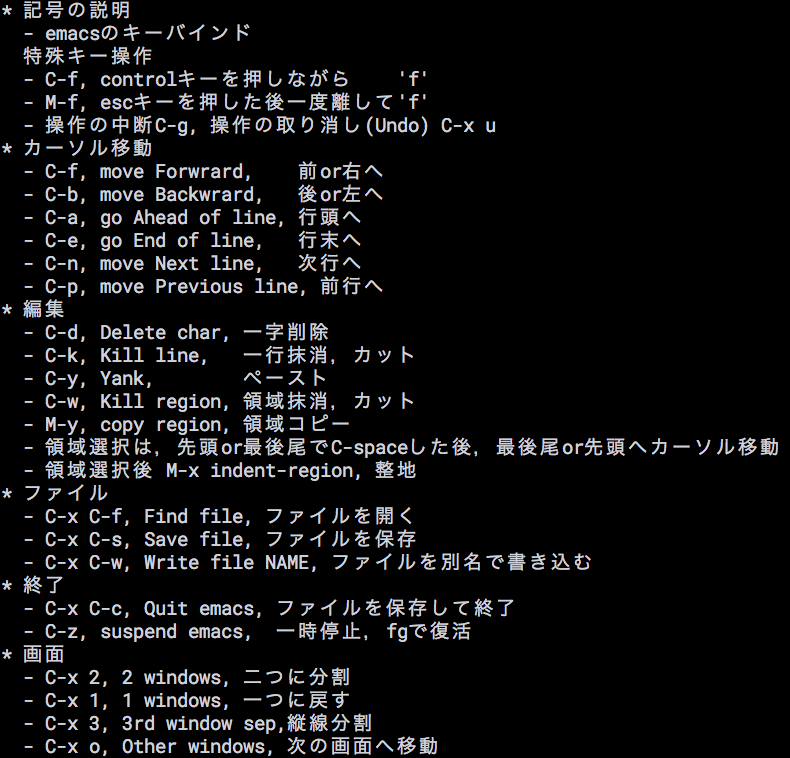
\includegraphics[width=100mm]{../../picture/keybind_string.png}
\end{center}
\caption{emacsキーバインドの文字表示.\label{keybind_string}}
\end{figure}

\subsection{image}\label{image}
各種キーバインドを画像で表示するオプション.キーバインドが視覚的に表現されているため,初学者にとってイメージしやすい表示となっている.しかし,画像表示のために新規ウィンドウが立ち上がるのでウィンドウ操作はマウスでなければならない場合がある.実際にコマンドを実行した場合に表示されるキーバインドの画像を以下に記す.
\begin{figure}[H]
\centering
\begin{center}
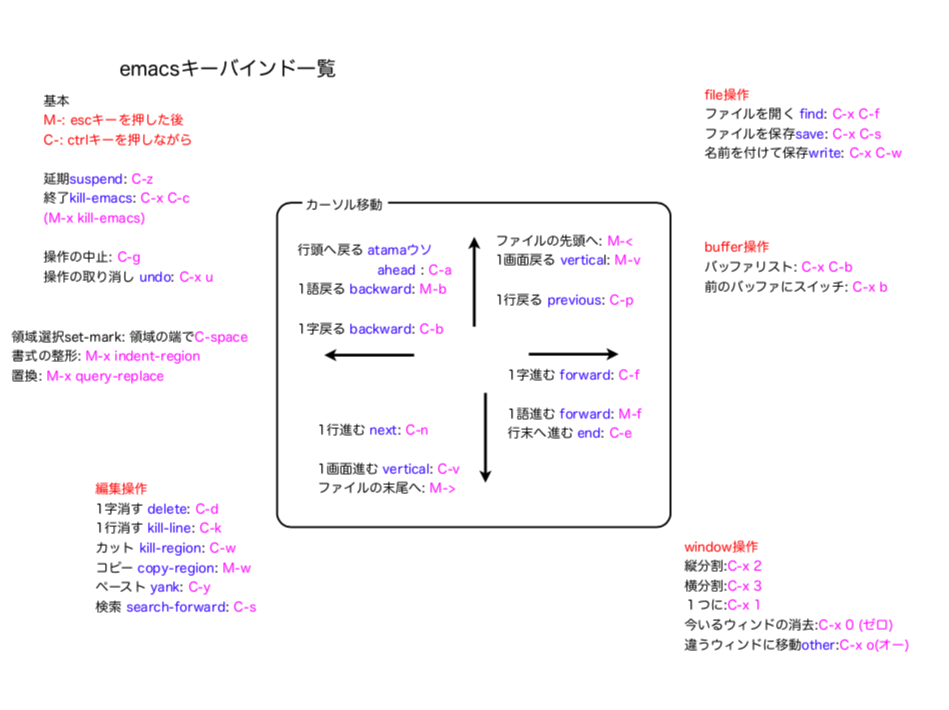
\includegraphics[width=150mm]{../../picture/keybind_image.png}
\end{center}
\caption{emacsキーバインドの文字表示.\label{keybind_image}}
\end{figure}

\section{theme}\label{theme}
sequential\_checkのnormal\_modeで使用するemacsのテーマの変更が可能.現在のテーマは黒と白の2種類から選ぶことができる.
